% The open set of the parabola V(y-x^2) obtained by deleting the point (1,1).
% Source: book/tex/alg-geom/zariski.tex (§ The Zariski topology on affine varieties).
\documentclass[border=2mm]{standalone}
\usepackage{tikz}\usepackage{amssymb}
\begin{document}
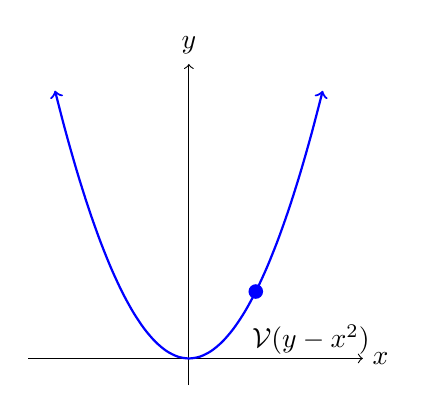
\begin{tikzpicture}[scale=0.85]
  \draw[->] (-2.4,0) -- (2.6,0) node[right] {$x$};
  \draw[->] (0,-0.4) -- (0,4.4) node[above] {$y$};
  \draw[blue,thick,<->] plot[domain=-2:2,smooth] (\x,{\x*\x});
  \node[below right] at (0.8,0.64) {$\mathcal V(y-x^2)$};
  \draw[fill=white,blue,line width=1pt] (1,1) circle (2.5pt);
\end{tikzpicture}
\end{document}
